\chapter{Inledning}

Det synliga universums massa består av mellan 70\% och 80\% väte. På grund av gravitation ansamlas vätet i vätemoln av olika storlekar. Vårt arbete utnyttjar en välkänd mekanism hos väte, en så kallad ''Spin-Flip Transition''\autocite{swin.edu:spin-flip}. Väteatomer består av en proton och en elektron. Dessa partiklar har en kvantmekanisk spin (som kallas spin även om partiklarna inte snurrar enligt den klassiska fysikens definition av spin). I basläget (det läge med lägst energinivå) har elektronen och protonen motsatt spin mot varandra. Om elektronen i väteatomen tar emot energi (vilket kan ske spontant genom exempelvis kollisioner mellan atomer) kan elektronen byta spin och få samma spin som protonen. Detta läge har marginellt högre energinivå än basläget. Om elektronen sedan byter till motsatt spin igen kommer överskottsenergin avges i form av en foton med en våglängd på ungefär 21cm. Denna våglängd kan vi observera med hjälp av ett radioteleskop här på jorden.

\section{Dopplereffekten}
Alla vågrörelser påverkas av dopplereffekten\autocite{nasa:doppler}. Dopplereffekten uppstår när en sändare som skickar ut någon form av vågrörelse har en hastighet riktad antingen mot eller från mottagaren. Om sändaren rör sig bort från mottagaren kommer våglängden bli längre (vågen ''sträcks ut'') och om sändaren rör sig mot mottagaren blir vågländen kortare (vågen ''trycks ihop''). 

I vår vardag upplevs dopplereffekten mest med ljudvågor. Om en observatör lyssnar på ett utryckningsfordon som åker förbi med sirenerna på kommer observatören notera att ljudet låter ljusare när sirenerna närmar sig och när sirenerna passerat observatören kommer ljudet låta mörkare. Givet formeln för dopplereffekten \autocite{wikipedia:doppler} 
\begin{equation*}
    \frac{f}{v_{wr}} = \frac{f_0}{v_{ws}}
\end{equation*}
kan vi räkna ut den upplevda  förskjutningen $x$ i frekvens genom 
\begin{align*}
    f &= f_0 \cdot x \\
    f &= \frac{f_0 \cdot v_{wr}}{v_{ws}} \Rightarrow x = \frac{v_{wr}}{v_{ws}}.
\end{align*}

Om vi tänker oss en ambulans med en hastighet 30m/s och en uppskattad ljudhastighet i luft på 300m/s kommer sirenens frekvens dopplerförskjutas till $f_0 \cdot \frac{300}{300-30}$, alltså 10\% högre än den sändes ut med. Ljuset som skickas ut från ambulansens varningsljus kommer också förskjutas men på grund av ljusets höga hastighet (runt 300 000 000 m/s) kommer ljusets frekvens endast öka med ungefär 0,00001\%.

\begin{figure}
    \centering
    \includegraphics{pics/atmo.jpg}
    \caption{Atmosfärens genomskinlighet för olika våglängder av ljus.}
    \label{fig:atmo_transparent}
\end{figure}

\section{Att observera rymden}
Förutom radiovågor görs astronomiska observationer på gamma- och röntgen-strålning, ultraviolett strålning, synligt ljus, infraröd strålning samt mikrovågor. Av dessa olika typer av ljus släpps enbart synligt ljus och radiovågor genom atmosfären (se figur \ref{fig:atmo_transparent}). Radiovågor passerar relativt ostört genom hela atmosfären \autocite{nasa:radiowaves}, så även om synligt ljus passerar störs det lätt av exempelvis moln \autocite{wikipedia:astro_seeing}. För övriga signaltyper används istället diverse satelliter i omloppsbana kring jorden.

\begin{figure}
    \centering
    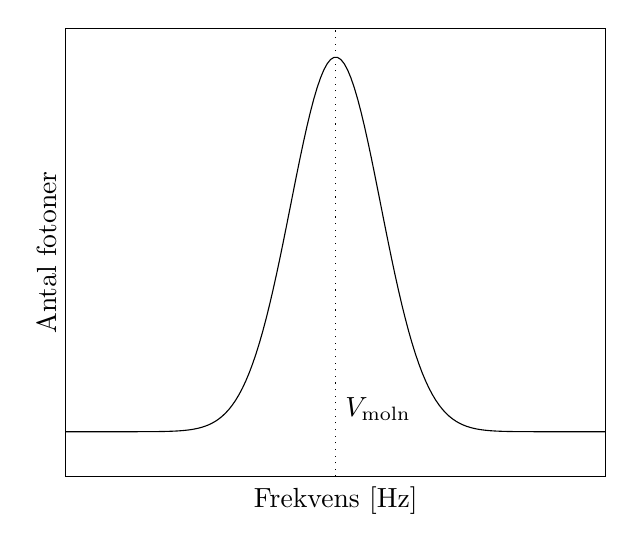
\begin{tikzpicture}
        \begin{axis}[
            ticks=none,
            ylabel=Antal fotoner, ylabel near ticks,
            xlabel={Frekvens [Hz]}, xlabel near ticks,
            xmin=-20, xmax=20,
            ymin=-1, ymax=9
        ]
        \addplot [domain=-25:25, samples=200]{1/0.3*(2*pi)^0.5 * exp(-((x)^2)/2*0.09)};
        \addplot [black, dotted] coordinates {
            (0,-1)
            (0,9)
        };
        \coordinate [label=right:$V_{\mathrm{moln}}$] (v-label) at (0,0.5);
        \end{axis}
    \end{tikzpicture}
    \caption{En exempelmätning med ett observerat vätemoln.}
    \label{fig:single_cloud}
\end{figure}

När vi gör en observation mäter vi i praktiken antalet fotoner inom ett visst spann av våglängder. Om vi tänker oss väte ansamlat i ''moln'' av olika storlekar i Vintergatan kommer molnet ha en viss hastighet med en riktning som följer Vintergatans rotation. Däremot kommer de enskilda atomerna som skickar ut fotonerna vi mäter ha olika relativa hastigheter där några kommer åka lite mer mot oss och några lite mer bort från oss. På grund av detta kommer antalet fotoner med olika våglängder spridas ut över ett visst intervall, men en majoritet av fotonerna kommer vara relativt stilla gentemot molnet (se figur \ref{fig:single_cloud}).

\begin{figure}%
    \centering
    \subfloat[]{
        \centering
        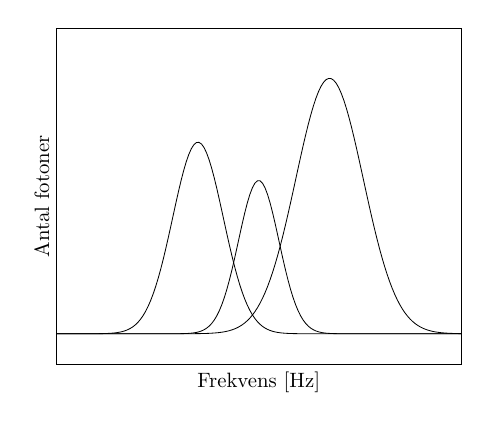
\begin{tikzpicture}[scale=0.75]
            \begin{axis}[
                ticks=none,
                ylabel=Antal fotoner, ylabel near ticks,
                xlabel={Frekvens [Hz]}, xlabel near ticks,
                xmin=-20, xmax=20,
                ymin=-1, ymax=10
            ]
                \addplot [domain=-25:25, samples=200, forget plot] {1/0.5*(2*pi)^0.5 * exp(-((x)^2)/2*0.25)};
                \addplot [domain=-25:25, samples=200, forget plot] {1/0.3*(2*pi)^0.5 * exp(-((x-7)^2)/2*0.09)};
                \addplot [domain=-25:25, samples=200, forget plot] {1/0.4*(2*pi)^0.5 * exp(-((x+6)^2)/2*0.16)};
            \end{axis}
        \end{tikzpicture}%
    }\qquad
    \subfloat[]{
        \centering
        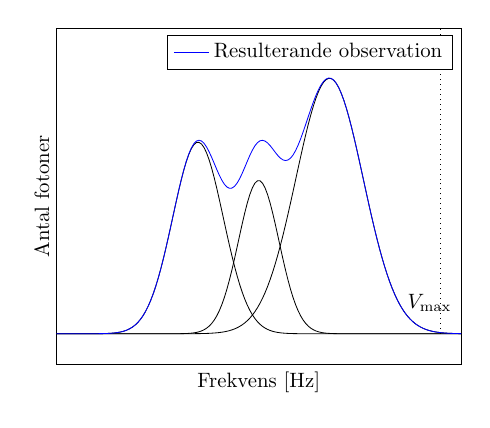
\begin{tikzpicture}[scale=0.75]
            \begin{axis}[
                ticks=none,
                ylabel=Antal fotoner, ylabel near ticks,
                xlabel={Frekvens [Hz]}, xlabel near ticks,
                xmin=-20, xmax=20,
                ymin=-1, ymax=10
            ]
                \addplot [domain=-25:25, samples=200, forget plot] {1/0.5*(2*pi)^0.5 * exp(-((x)^2)/2*0.25)};
                \addplot [domain=-25:25, samples=200, forget plot] {1/0.3*(2*pi)^0.5 * exp(-((x-7)^2)/2*0.09)};
                \addplot [domain=-25:25, samples=200, forget plot] {1/0.4*(2*pi)^0.5 * exp(-((x+6)^2)/2*0.16)};
                \addplot [blue,domain=-25:25, samples=200] {(1/0.5*(2*pi)^0.5 * exp(-((x)^2)/2*0.25)) + (1/0.3*(2*pi)^0.5 * exp(-((x-7)^2)/2*0.09)) + (1/0.4*(2*pi)^0.5 * exp(-((x+6)^2)/2*0.16))};
                \addlegendentry{Resulterande observation}
                \addplot [black, dotted] coordinates {
                    (18,0)
                    (18,12)
                };
                \coordinate [label=right:$V_{\mathrm{max}}$] (v-max) at (14,1);
            \end{axis}
        \end{tikzpicture}%
    }
    \caption{En exempelmätning med tre observerade vätemoln.}
    \label{fig:multiple_clouds}
\end{figure}

I figur \ref{fig:multiple_clouds}a har tre vätemoln observerats. I de fall mer än ett vätemoln observerats får observatören själv räkna ut hur många moln som observerats och hur de originella observationskurvorna såg ut, se figur \ref{fig:multiple_clouds}b.

\subsection{Koordinatsystem}
Många galaxer, även Vintergatan, har en skivform där merparten av den synliga massan återfinns längs med skivans plan. Det är möjligt att använda detta plan som bas för ett koordinatsystem där koordinaterna motsvarar en linje längs med alla tre dimensionerna\autocite{swin:galactic_coords}. Linjen vid longitud och latitud noll går genom Vintergatans mitt. Hela koordinatsystemet utgår från solsystemet. Se figur \ref{fig:galactic_coords}

\begin{figure}
    \centering
    \includegraphics[width=0.8\textwidth]{pics/galactic_coords.jpg}
    \caption{Det galaktiska koordinatsystemet.}
    \label{fig:galactic_coords}
\end{figure}

\section{Syfte}
Syftet med den här rapporten är att besvara följande frågeställning: Hur ser Vintergatans galaktiska struktur ut? Därpå kommer vi även undersöka hur galaktiska strukturer uppstår, däremot kommer inget slutgiltigt svar att erbjudas på den andra frågan.